% Presentation: Introduction to MOM
%     Location: CoE CMS Winter School, 12 July 2012
%       Author: Marshall Ward
%-----------------------------------------------------------------------------%
\documentclass{beamer}

% Font configuration
\usepackage{pxfonts}

% Packages
\usepackage{hyperref}
\usepackage[textstyle, squaren]{SIunits}
\usepackage{textpos}

\usepackage{color}
\definecolor{ltblue}{rgb}{0.9, 0.9, 1.0}
\definecolor{dkgreen}{rgb}{0.0, 0.6, 0.0}
\definecolor{gray}{rgb}{0.5, 0.5, 0.5}
\definecolor{mauve}{rgb}{0.58, 0.0, 0.82}

% Solarized colors
\definecolor{base03}{rgb}{0.0, 0.17, 0.21}
\definecolor{base01}{rgb}{0.35, 0.43, 0.46}
\definecolor{base0}{rgb}{0.51, 0.58, 0.59}

% Beamer configuration
\usetheme{Frankfurt}
\AtBeginSection[]{
    \frame<beamer>{\tableofcontents[current]}
}

% LaTeX configuration
\graphicspath{{figures/}}

% Listings configuration
\usepackage{listings}
\lstset{
    language=bash,
    moredelim=[s][\color{mauve}]{\$\{}{\}},
    showspaces=false,
    showstringspaces=false,
    %basicstyle=\ttfamily\color{base0},
    %backgroundcolor=\color{base03},
    basicstyle=\ttfamily,
    backgroundcolor=\color{ltblue},
    numberstyle=\tiny\color{gray},
    keywordstyle=\color{blue},
    commentstyle=\color{dkgreen},
    stringstyle=\color{mauve},
}

%=============================================================================%
\title{An Introduction to MOM}
\author{Marshall Ward}
\institute{Australian National University\\Research School of Earth Sciences}
\date{12 July 2012}

%=============================================================================%
\begin{document}
\begin{frame}
    \titlepage
    % Place logos
    \begin{textblock*}{0.5\textwidth}(-0.05\textwidth, -0.81\textheight)
        
\includegraphics[width=\textwidth]{coecms_logo.pdf}
    \end{textblock*}
    \begin{textblock*}{0.15\textwidth}(0.88\textwidth, -0.81\textheight)
        
\includegraphics[width=\textwidth]{arc_logo.pdf}
    \end{textblock*}
    \begin{textblock*}{\textwidth}(0\textwidth, 0.02\textheight)
        
\includegraphics[height=0.063\textheight]{anu_logo.pdf}
        \hspace{0.02\textwidth}
        
\includegraphics[height=0.063\textheight]{monash_logo.png}
        \hspace{0.02\textwidth}
        
\includegraphics[height=0.061\textheight]{umelb_logo.png}
        \hspace{0.02\textwidth}
        
\includegraphics[height=0.061\textheight]{unsw_logo.jpg}
        \hspace{0.02\textwidth}
        
\includegraphics[height=0.061\textheight]{utas_logo.jpg}
    \end{textblock*}
\end{frame}

%=============================================================================%
\section[Overview]{MOM4 Overview}

%-----------------------------------------------------------------------------%
\begin{frame}
    \frametitle{MOM: The Modular Ocean Model}

    \begin{columns}
        \column{0.65\textwidth}
        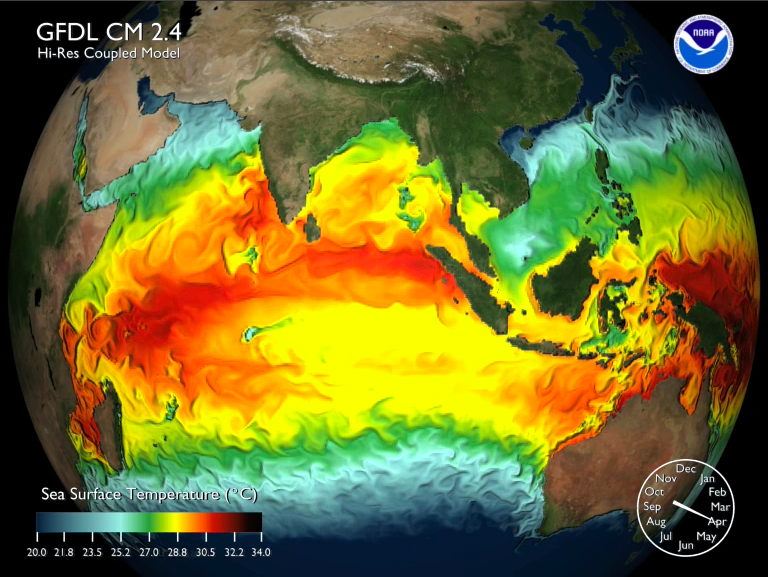
\includegraphics[width=\textwidth]{hires_indian_sst.jpg}
        \column{0.35\textwidth}
        \begin{itemize}
            \item GFDL Ocean Climate Model (Princeton, USA)
            \item Nearly 50-year development history
            \item Maintainer: Stephen Griffies
        \end{itemize}
    \end{columns}
    \vspace{10pt}
    {\tiny \lstinline|http://www.gfdl.noaa.gov/pix/tools_and_data/fms/hires_indian_sst.jpg|}
\end{frame}

%-----------------------------------------------------------------------------%
\begin{frame}
    \frametitle{MOM4 Dynamic Core}
    
    \begin{itemize}
        \item Hydrostatic, Boussinesq
        \item Orthogonal Horizontal Grids
        \item Generalised vertical grids
		\item Explicit free surface
		\item Modern thermodynamic support
        \item Partial grid topograpy
    \end{itemize}
\end{frame}

%-----------------------------------------------------------------------------%
\begin{frame}
    \frametitle{Orthogonal Horizontal Grids}
    
    \begin{center}
        \includegraphics<1>[width=0.7\textwidth]{merc_tripolar.pdf}
        \includegraphics<2>[width=0.5\textwidth]{nh_tripolar.pdf}
        \includegraphics<2>[width=0.5\textwidth]{sh_tripolar.pdf}
        %\includegraphics<3>[width=0.7\textwidth]{merc_auscom.pdf}
    \end{center}
\end{frame}

%-----------------------------------------------------------------------------%
\begin{frame}
    \frametitle{MOM4 grid layout}

    \begin{columns}
        \column{0.5\textwidth}
        \begin{center}
            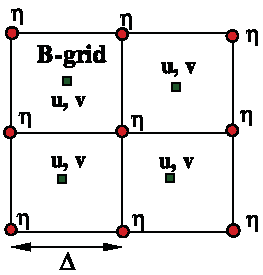
\includegraphics[width=\textwidth]{b_grid.pdf}
        \end{center}
        \column{0.5\textwidth}
        \begin{itemize}
            \item Arakawa ``B-grid''
            \item Tracers ($\rho$, $T$, $S$, etc.) on cell centres
            \item Velocities ($u$, $v$) on cell corners
            \item ``Supergrids'' are half-$\Delta$ resolution
        \end{itemize}
    \end{columns}
    {\tiny Rajpoot, Bhaumik, Sengupta (2011)}
\end{frame}

%-----------------------------------------------------------------------------%
\begin{frame}
    \frametitle{Generalised Vertical Grids}
    
    Several vertical coordinates are supported:
    \begin{description}
        \item[$z$] Geopotential ($\approx$ depth, Boussinesq)
        
        \item[$p$] Hydrostatic pressure (Non-Boussinesq)
        
        \item[$z^*$, $p^*$] Quasi-horizontal vertical grids
            $$
            z^* = H(\mathbf{x}) \left(\frac{z - \eta}{H + \eta}\right)
            $$
        \item[$\sigma^{(z)}, \sigma^{(p)}$] Terrain-following coordinates
            $$
            \sigma^{(z)} = \frac{z - \eta}{H + \eta}
            $$
            ($\sigma$ not recommended for complex flows)
    \end{description}
\end{frame}

%-----------------------------------------------------------------------------%
\begin{frame}
    \frametitle{Quasi-horizontal Vertical Grids}
    
    \begin{center}
        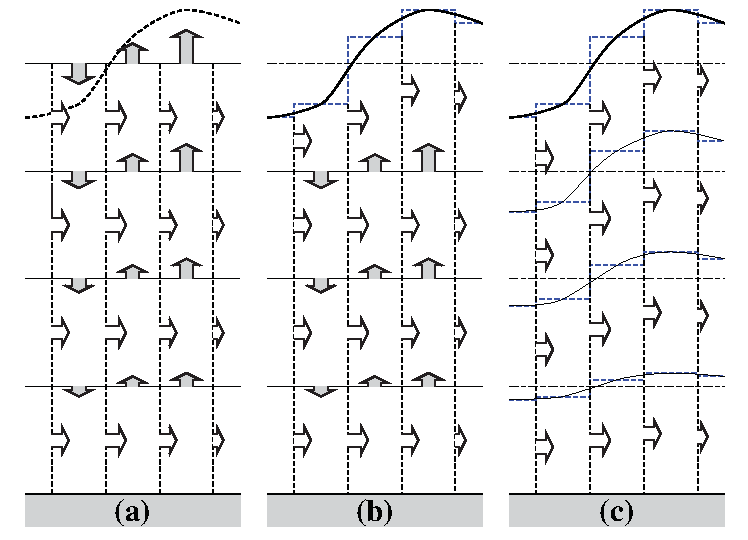
\includegraphics[width=0.8\textwidth]{zstar.pdf}
    \end{center}
    
    {\tiny "NEMO Ocean Engine", Madec et al. (2012)}
\end{frame}

%-----------------------------------------------------------------------------%
\begin{frame}
    \frametitle{Alternative Ocean Models}
    
    Qualitatively different models
    \begin{description}
        \item[MITgcm] nonhydrostatic, finite volume
        \item[GOLD] isopycnal ($\rho$ vertical grid)
        \item[ROMS] ``regional'' ($\sigma$ vertical grid)
        \item[HYCOM] ``hybrid'' vertical grid ($z$-$\rho$-$\sigma$)
    \end{description}
    
    "MOM-like" (Bryan-Cox) Ocean Models
    \begin{description}
        \item[NEMO] C-grid
        \item[POP2] (part of CESM)
        \item[COCO] (part of MIROC)
    \end{description}
\end{frame}

%=============================================================================%
\section{MOM4 Quick User's guide}
%-----------------------------------------------------------------------------%
\begin{frame}[fragile]
    \frametitle{Acquiring the source code}
    
    Up-to-date versions of the source code are available on a subversion (svn)
    server hosted by NCI:
    
    \begin{lstlisting}
# Enter as one line
svn co https://access-svn.nci.org.au/mom4
               /branches/local_changes
    \end{lstlisting}
    For access: \lstinline|climate_help@nf.nci.org.au|
    
    \textit{IP address required} 
\end{frame}

%-----------------------------------------------------------------------------%
\begin{frame}[fragile]
    \frametitle{Source Code Versions}
    
    Major source code branches:
    \begin{description}
        \item[\ttfamily{mom4/trunk}] GFDL code release mirror\\
                                     Unconfigured for NCI\\
                                     \textit{MOM4.1 (Dec 2009)}
        \item[\ttfamily{local\_changes}] Stable release on vayu\\
                                         Pre-configured for NCI\\
                                         \textit{MOM4.1 (Dec 2009)}
        \item[\ttfamily{future\_local\_changes}] Experimental release on vayu\\
                                                 Pre-configured for NCI\\
                                                 \textit{MOM4.2 Beta}
    \end{description}

    \textit{Note: This format may change in the future}
\end{frame}

%-----------------------------------------------------------------------------%
\begin{frame}[fragile]
    \frametitle{MOM4 Library Dependencies}

    The following libraries and applications are recommended:
    \begin{description}
        \item[\ttfamily{pbs}] Queueing system (usually included)
        \item[\ttfamily{intel-fc}] Intel Fortran Compiler
        \item[\ttfamily{intel-cc}] Intel C Compiler
        \item[\ttfamily{intel-mkl}] Intel Math Libraries
        \item[\ttfamily{openmpi}] MPI Parallelisation
        \item[\ttfamily{hdf5}] File I/O backend
        \item[\ttfamily{netcdf}] File I/O API \\
            (For MOM4.2, use \ttfamily{netcdf/4.1.2})
        \item[\ttfamily{ncview}] Simple netCDF4 data viewer
    \end{description}
\end{frame}

%-----------------------------------------------------------------------------%
\begin{frame}[fragile]
    \frametitle{MOM4 Library Dependencies}
    
    On NCI machines, use environment modules:
    \begin{lstlisting}
> module load intel-fc
> module load netcdf/4.1.2
# etc...
    \end{lstlisting}
    Most scripts handle this automatically, but occasionally you must do it
    manually. 

    \vspace{10pt}

    To automatically import at login, add the commands to your
    \lstinline|.login| file (or \lstinline|.profile| if using
    \lstinline|bash|).
\end{frame}

%-----------------------------------------------------------------------------%
\begin{frame}[fragile]
    \frametitle{Compiling MOM}
    
    Most repositories have pre-configured build scripts for vayu:
    \begin{lstlisting}
# From source directory
> cd exp
> qsub mom4p1_solo_compile.sh
    \end{lstlisting}
    
    Default executable path:
    \begin{lstlisting}
> /short/${PROJECT}/${USER}/mom4/exec_vayu
     /mom4p1_solo/fms_mom4p1_solo.x
    \end{lstlisting}
    
    Compilation should take approximately 10 minutes. 
\end{frame}

%-----------------------------------------------------------------------------%
\begin{frame}
    \frametitle{Creating a model grid}
    
    Mosaic grid generation for ocean-only (\textit{solo}) simulations:
    \begin{itemize}
        \item Vertical grid
        \item Horizontal grid
        \item Mosaic manifest file
        \item Topography
    \end{itemize}
    
    Caveats:
    \begin{itemize}
        \item ``Supergrid'' output: $N$ cells, $2N+1$ grid points
        \item New toolset, differs from previous grid format
        \item Mosaic is mostly finished, but still under development
    \end{itemize}
\end{frame}

%-----------------------------------------------------------------------------%
\begin{frame}[fragile]
    \frametitle{Vertical Grid Generation}
    
    Uniform vertical grid:
    \begin{lstlisting}
# From the source directory
> cd src/tools/make_vgrid
> make
> ./make_vgrid \
     --nbnds 3 \
     --bnds 0,4000 \
     --nz 40
    \end{lstlisting}
    
    Variable resolution:
    \begin{lstlisting}
> ./make_vgrid \
     --nbnds 4 \
     --bnds 0,100,500,4000 \
     --nz 10,10,20
    \end{lstlisting}
\end{frame}
%-----------------------------------------------------------------------------%
\begin{frame}[fragile]
    \frametitle{Horizontal Grid Generation}
   
    Uniform $1^\circ$ spherical grid:
    \begin{lstlisting}
> cd src/tools/make_hgrid
> make
> ./make_hgrid \
     --grid_type regular_lonlat_grid \
     --nxbnd 2 \
     --nybnd 2 \
     --xbnd 0,40 \
     --ybnd -80,80 \
     --nlon 40 \
     --nlat 160
    \end{lstlisting}
\end{frame}

%-----------------------------------------------------------------------------%
\begin{frame}[fragile]
    \frametitle{Mosaic manifest file}
    
    \textit{Mosaic} files contain metadata to grid files:
    \begin{lstlisting}
> cd src/tools/make_solo_mosaic
> make
> ./make_solo_mosaic \
     --num_tiles 1 \
     --dir . \
     --periodx 40
    \end{lstlisting}
\end{frame}

%-----------------------------------------------------------------------------%
\begin{frame}[fragile]
    \frametitle{Topography generation}
   
    Idealised flat-bottom topography
    \begin{lstlisting}
> cd src/tools/make_topog
> make
> ./make_topog \
     --mosaic solo_mosaic.nc \
     --topog_type rectangular_basin \
     --basin_depth 4000
    \end{lstlisting}

    Note: For the parallel MPI version, use
    \begin{lstlisting}
> make -f Makefile_mpi
    \end{lstlisting}
\end{frame}

%-----------------------------------------------------------------------------%
\begin{frame}
    \frametitle{Interpolated Topography}
    
    Parallel job submission example:
    \lstinputlisting{scripts/interp_topog.sh}
\end{frame}

%-----------------------------------------------------------------------------%
\begin{frame}
    \frametitle{Model Configuration}
    
    MOM4 configuration files:
    \begin{description}
        \item[\ttfamily{input.nml}] Major configuration settings (Fortran
            namelist)
        \item[\ttfamily{diag\_table}] Diagnostic output
        \item[\ttfamily{data\_table}] Input fields and boundary conditions
        \item[\ttfamily{field\_table}] Initial conditions, advection
            configuration
    \end{description}
\end{frame}

%-----------------------------------------------------------------------------%
\begin{frame}[fragile]
    \frametitle{Running MOM}
    
    To run MOM from the terminal:
    \begin{lstlisting}
> mkdir ${expt}
> cp ${myconfig}/input.nml ${expt}
> cp ${myconfig}/*_table ${expt}
> mkdir ${expt}/INPUT
> mkdir ${expt}/RESTART
# Link (or copy) grids, mosaics, data to INPUT
> ln -s ${mydata}/*.nc ${expt}/INPUT
> ./${mom_executable}
    \end{lstlisting}

\end{frame}

%-----------------------------------------------------------------------------%
\begin{frame}[fragile]
    \frametitle{Running MOM}
    
    To submit MOM on vayu:
    \begin{lstlisting}
> cd ${mom_code}
> mkdir work/${expt}
> mkdir work/${expt}/INPUT
> cp ${myconfig}/input.nml work/${expt}/INPUT
> cp ${myconfig}/*_table work/${expt}/INPUT
> cp ${mydata}/*.nc ${firstrun}/INPUT
> cd exp
> qsub mom4p1_solo_run.csh
    \end{lstlisting}
The script \lstinline|mom4p1_solo_run| will require further configuration.

\end{frame}

%-----------------------------------------------------------------------------%
\begin{frame}[fragile]
    \frametitle{Setting the run time}
   
    \lstinline|input.nml|:
    \lstinputlisting[language=fortran]{scripts/run_time.nml}
\end{frame}

%-----------------------------------------------------------------------------%
\begin{frame}[fragile]
    \frametitle{Timestep configuration}
   
    \lstinline|input.nml|:
    \lstinputlisting[language=fortran]{scripts/timestep.nml}
    60 free surface (\textit{barotropic}) timesteps for each model
    (\textit{baroclinic}) timestep
\end{frame}

%-----------------------------------------------------------------------------%
\begin{frame}[fragile]
    \frametitle{MOM4 Diagnostics}
    
    \lstinline|diag_table| file record:
    \begin{lstlisting}
"ocean_snap", 5,"days", 1,"days", "Time"
    \end{lstlisting}
    \begin{itemize}
        \item \lstinline|"ocean_snap"|: Output filename
        \item \lstinline|1, "days"|: Output snapshot frequency
        \item \lstinline|1, "days"|: Output units
        \item \lstinline|"Time"|: Output time axis label
    \end{itemize}
    Several output files can be registered, each containing different
    variables.
\end{frame}

%-----------------------------------------------------------------------------%
\begin{frame}[fragile]
    \frametitle{MOM4 Diagnostics}
    
    \lstinline|diag_table| field record:
    \begin{lstlisting}
"ocean_model", "u", "u", "ocean_snap", "all",
    .false., "none", 2
    \end{lstlisting}
    \begin{itemize}
        \item \lstinline|"ocean_model"|: MOM4 module containing the variable
        \item \lstinline|"u", "u"|: Variable name (MOM4 name, output name)
        \item \lstinline|"ocean_snap"|: Registered output file
        \item \lstinline|"all"|: Grid sampling rate
        \item \lstinline|.false.|: Average between snapshots
        \item \lstinline|"none"|: Generic option flag (rarely used)
        \item \lstinline|2|: output data type (1: double, 2: float)
    \end{itemize}
\end{frame}

%-----------------------------------------------------------------------------%
\begin{frame}[fragile]
    \frametitle{Pre-configured MOM4 Runs}
    
    Available at
    {\small
    \lstinline|ftp://ftp.gfdl.noaa.gov/perm/MOM4/mom4p1_pubrel_dec2009/exp/|}
    
    \vspace{10pt}

    Ocean-only experiments:
    \begin{description}
        \item[\ttfamily{torus1}] Tracer advection test
        \item[\ttfamily{symmetric\_box1}] Re-entrant channel, symmetric winds
        \item[\ttfamily{box1}] Thermohaline test
        \item[\ttfamily{gyre1}] Basin gyre test
        \item[\ttfamily{dome1}] \textbf{DOME} overflow experiment
        \item[\ttfamily{iom1}] Indian Ocean model
    \end{description}
    
    Coupled experiments:
    \begin{description}
        \item[\ttfamily{om3core3}] Global ocean model
        \item[\ttfamily{CM2.1p1}] Global CMIP output
    \end{description}
\end{frame}

%=============================================================================%
\section{Numerical Grid Design}
%-----------------------------------------------------------------------------%
\begin{frame}
    \frametitle{Numerical Fidelity}
    
    Modellers would like to solve equations like this:
    $$
    \frac{\partial \phi}{\partial t} + c \frac{\partial \phi}{\partial x} = 0
    $$
    but computers can only solve equations like this:
    $$
    \phi^{n+1}_i = \phi^n_i + c \Delta t
        \left(\frac{\phi^n_{i+1} - \phi^n_{i-1}}{2\Delta x_i} \right)
    $$
    Grid sizes $\Delta x$, $\Delta t$ are the primary measures of convergence.
\end{frame}

%-----------------------------------------------------------------------------%
\begin{frame}
    \frametitle{Scales of the Ocean}
    
    \begin{center}
        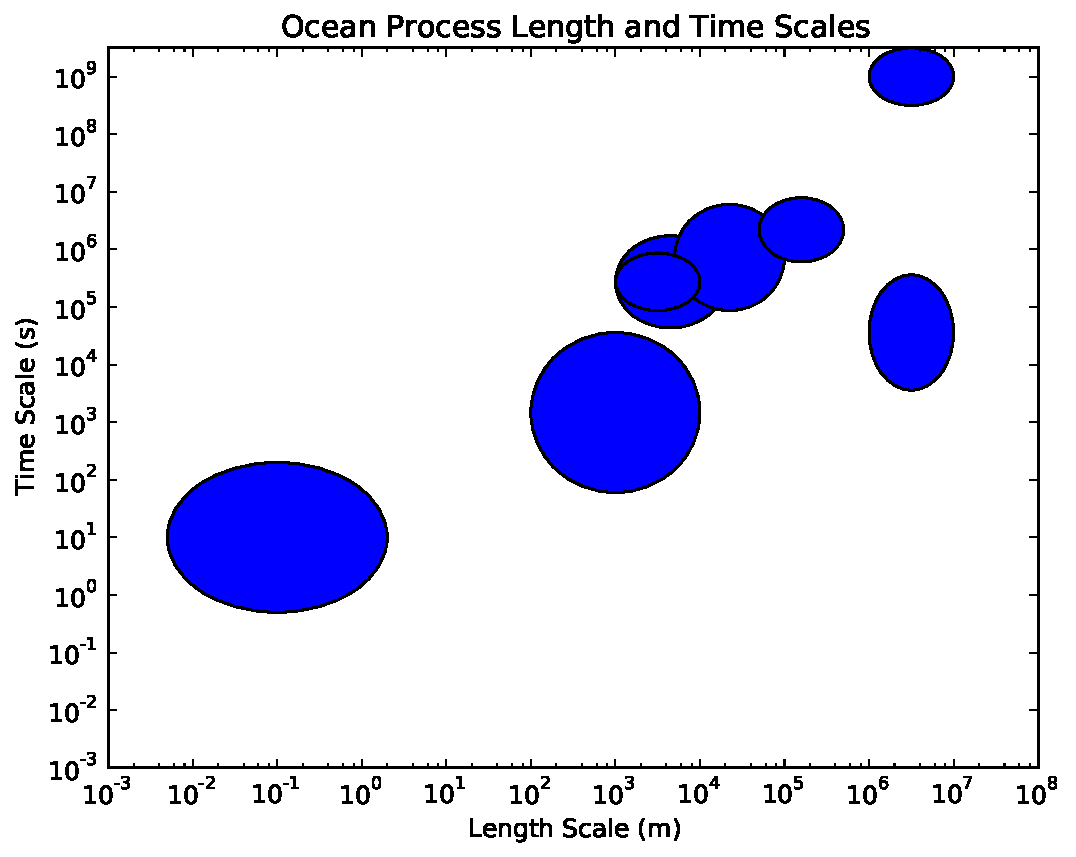
\includegraphics[width=0.75\textwidth]{ocean_scales.pdf}
    \end{center}
    
    {\tiny Adapted from:\\
        Cushman-Roisin, Beckers (2011), Talley, Pickard, Emery, Swift (2011)}
\end{frame}

%-----------------------------------------------------------------------------%
\begin{frame}
    \frametitle{How long to compute everything?}
    
    Largest scales (global, millenial scale) in terms of smallest:
    \begin{itemize}
        \item Horizontal scales: $L \sim 10^{11}$
        \item Vertical scales: $H \sim 10^7$
        \item Timescales: $T \sim 10^{14}$
    \end{itemize}
    Computations: $N \sim L^2 H T \sim 10^{43}$
    
    \vspace{10pt}
    
    In the petaflop era ($10^{16}$ flops, 10 petaflops):
    \begin{itemize}
        \item $T \sim 10^{27}$ seconds
    \end{itemize}
    (Age of the universe: $\sim 10^{17}$ seconds)
\end{frame}

%-----------------------------------------------------------------------------%
\begin{frame}
    \frametitle{More typical computation numbers}
    
    Current models only resolve the biggest scales:
    \begin{itemize}
        \item Horizontal scales: $L \sim 10^3$
        \item Vertical scales: $H \sim 10^2$
        \item Timescales: $T \sim 10^{8}$
    \end{itemize}
    Computations: $N \sim L^2 H T \sim 10^{16}$
    
    \vspace{10pt}
    
    Hardware limits lead to gigaflop speeds ($10^{10}$) per job:
    \begin{itemize}
        \item $T \sim 10^{6}$ seconds (or months)
    \end{itemize}
    (Don't take any of these numbers too seriously!)
\end{frame}

%-----------------------------------------------------------------------------%
\begin{frame}
    \frametitle{Designing a grid}
    
    Rough guide for designing a grid:
    \begin{itemize}
        \item Choose the spatial resolution $\Delta x$
        \item Identify the important physical processes
        \item Estimate the required $\Delta t$ for stability
        \item Apply dissipations to the smallest scales
        \item Reduce or increase $\Delta t$ and dissipations until it runs
    \end{itemize}
\end{frame}

%=============================================================================%
\section{Parameterization Overview}
%-----------------------------------------------------------------------------%
\begin{frame}
    \frametitle{Parameterization Overview}
    
    Partial List of MOM4 Parameterizations
    \begin{itemize}
        \item Vertical Mixing
        \item Mixed Layer
        \item Bottom Boundary Layer
        \item Neutral Physics
        \item Submesoscale
    \end{itemize}
\end{frame}

%-----------------------------------------------------------------------------%
\begin{frame}
    \frametitle{Turbulent Cascading}

    Explain the pumping of energy to smaller scales
\end{frame}

%-----------------------------------------------------------------------------%
\begin{frame}
    \frametitle{Laplacian and Biharmonic Viscosities}

    Illustrate scale-selective dissipation viscosities
\end{frame}

%-----------------------------------------------------------------------------%
\begin{frame}
    \frametitle{Friction and Turbulent Control}
    
    Laplacian (constant) friction models:
    $$
    F = A \nabla^2 \mathbf{u}
    $$
    For Smagorinsky viscosity:
    $$
    A = \left(\frac{C \Delta}{\pi}\right)^2 |D| + v \Delta
    $$
    where $\Delta$ is grid spacing and $|D|$ is strain rate
\end{frame}

%-----------------------------------------------------------------------------%
\begin{frame}
    \frametitle{Configuring Laplacian Viscosity}
    
    \begin{columns}
        \column{0.67\textwidth}
        \lstinputlisting[language=fortran]{scripts/lap_friction.nml}
        \column{0.32\textwidth}
        Constant:
        
        $A = \text{\lstinline|alap|}$
        
        \vspace{10pt}
        
        Smagorinsky:
        
        $C = \text{\lstinline|k_smag_iso|}$
        
        $v = \text{\lstinline|vel_micom_iso|}$
    \end{columns}
\end{frame}

%=============================================================================%
\section{Coupling}
%-----------------------------------------------------------------------------%
\begin{frame}
    \frametitle{MOM4 Coupling}
    
    \begin{itemize}
        \item FMS (GFDL)
        \item OASIS (ACCESS)
        \item SIS, CICE
    \end{itemize}
\end{frame}

%=============================================================================%
\end{document}
